\documentclass{beamer}

% Packages
\usepackage{graphicx}    % For including images
\usepackage{amsmath}     % For mathematical symbols
\usepackage{braket}      % For Dirac notation
\usepackage[absolute,overlay]{textpos}
\usepackage{amsmath}
% \usepackage{amsmath, amssymb, dsfont}
% \usepackage{algorithm}
% \usepackage{algorithmicx}
% \usepackage{enumitem}


\theoremstyle{definition}
\newtheorem{algorithm}{Algorithm}
\newtheorem{construction}[theorem]{Construction}

\newcommand\numberthis{\addtocounter{equation}{1}\tag{\theequation}}

\newcommand{\cas}{\mathrm{cas}}
\newcommand{\cht}{\mathsf{H}}
\newcommand{\qht}{\mathsf{QHT}}
\newcommand{\cft}{\mathsf{F}}
\newcommand{\qft}{\mathsf{QFT}}
\newcommand{\comph}{\mathsf{cmpIndex}}
\newcommand{\gen}{\mathsf{Gen}}
\newcommand{\ver}{\mathsf{Ver}}




% Title Information
\title{Quantum Walks and Applications to Quantum Money}
\author{Seyed Ali Mousavi}
\institute{Supervised by Dr. Jake Doliskani}
\date{\today}

\begin{document}

% Title Slide
\begin{frame}
    \titlepage
\end{frame}





\begin{frame}{Program and Courses Taken}

   
    
    \begin{textblock*}{12cm}(0.5cm,1.5cm)
       \begin{itemize}
        \item Program: M.A.Sc in Software Engineering
        \vspace{1cm}
        \item CAS 701,  Logic \& Discrete Mathematics
        \item COMPSCI 6TE3, Continuous optimization
        \item CAS 721, Combinatorics \& Computing
        \item CAS 741, Development of Scientific Computation Software
       \end{itemize}
    \end{textblock*}

    \title{SDSD}
    


\end{frame}







\begin{frame}{Seminars}
    
    \begin{textblock*}{12cm}(0.5cm,1.5cm)
       \begin{itemize}
        \item I have participated in 6 seminars during my program.
       \end{itemize}
    \end{textblock*}
    

\end{frame}




\begin{frame}{Poster}
    
    \begin{figure}
        \centering
        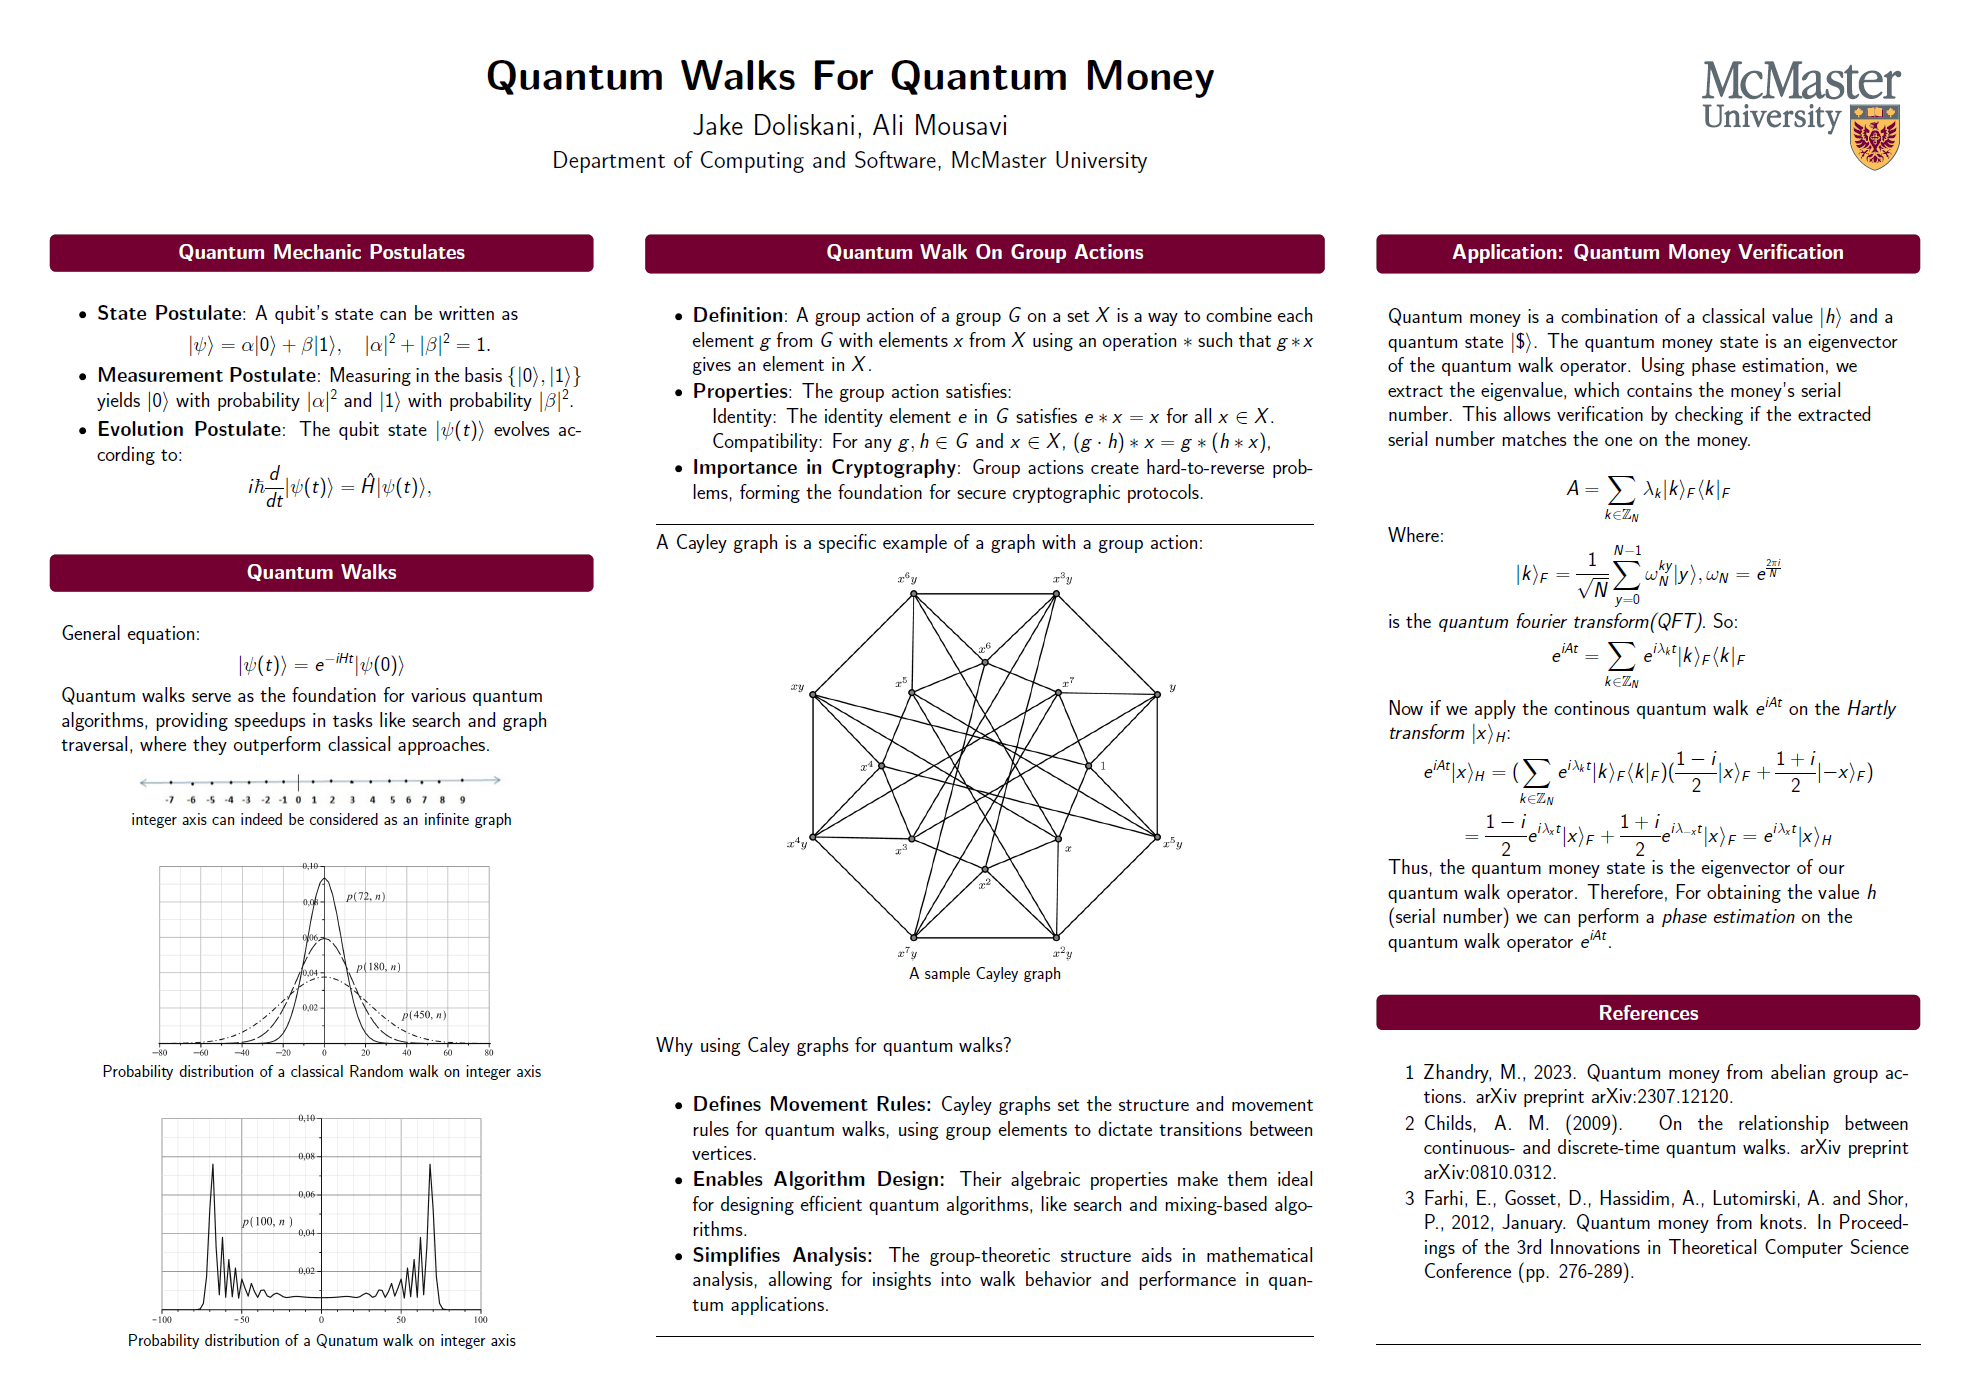
\includegraphics[width=1\textwidth]{poster.png}
        \caption{Presented at Nov. 6, 2024}
    \end{figure}

\end{frame}





\begin{frame}{The Hartley Transform}
    
    \begin{textblock*}{12cm}(0.5cm,1.5cm)
        item Let $N$ be a positive integer, and let $\mathbb{Z}_N$ be the additive cyclic group of integers modulo $N$. The Hartley transform of a function $f: \mathbb{Z}_N \to \mathbb{R}$ is the function $\cht_N(f): \mathbb{Z}_N \to \mathbb{R}$ defined by
        \[ \cht_N(f)(a) = \frac{1}{\sqrt{N}} \sum_{y = 0}^{N - 1} \cas\Big(\frac{2 \pi ay}{N}\Big) f(y),  \]
        where $\cas(x) = \cos(x) + \sin(x)$ \\
        For a single basis element of the cyclic group $\mathbb{Z}_N$, the quantum Hartly transform simplifies to
        \begin{equation}
            \label{eq:qht-N}
            \qht_N: \ket{a} \mapsto \frac{1}{\sqrt{N}} \sum_{y = 0}^{N - 1} \cas\Big(\frac{2\pi a y}{N}\Big) \ket{y}.
        \end{equation}
    \end{textblock*}
    

\end{frame}




\begin{frame}{An efficient new algorithm for QHT}
    
    \begin{textblock*}{12cm}(0.5cm,1.5cm)
        First, let us briefly explain how the algorithm for $\qft_N$ works:
        \begin{align*}
            \qft_N\ket{a}
            & = \frac{1}{\sqrt{N}} \sum_{y = 0}^{N - 1} \omega_N^{ay}\ket{y} \\
            & = \frac{1}{\sqrt{N}} \sum_{y = 0}^{N / 2 - 1} \omega_N^{ay} \ket{y} + (-1)^a \sum_{y = 0}^{N / 2 - 1} \omega_N^{ay} \ket{y + N/2} \\
            & = \frac{1}{\sqrt{N / 2}} \sum_{y = 0}^{N / 2 - 1} \omega_N^{ay} \frac{1}{\sqrt{2}} (\ket{0} + (-1)^a \ket{1}) \ket{y}, \numberthis\label{eq:qft_alt}
        \end{align*}
       
    \end{textblock*}
    

\end{frame}


\begin{frame}{An efficient new algorithm for QHT}
    
    \begin{textblock*}{12cm}(0.5cm,1.5cm)
        Let $\ket{a} = \ket{t}\ket{b}$, where $b$ is the least significant bit of $a$, so that $a = 2t + b$. Applying $\qft_{N / 2}$ to the first register, we obtain the state
        \[ \frac{1}{\sqrt{N / 2}} \sum_{y = 0}^{N / 2 - 1} \omega_N^{2ty} \ket{y} \ket{b}. \]
        Next, we apply the phase unitary $P(y, b): \ket{y} \ket{b} \mapsto \omega_N^{by} \ket{y} \ket{b}$, and finally, we apply a Hadamard transform to the last qubit. The result is the state in \eqref{eq:qft_alt}.  

    \end{textblock*}
    

\end{frame}



\begin{frame}{An efficient new algorithm for QHT}
    
    \begin{textblock*}{12cm}(0.5cm,1.5cm)
        \begin{equation}
            % \label{eq:cas-expand}
            \frac{1}{\sqrt{N}} \sum_{y = 0}^{N - 1} \cas\Big( \frac{2\pi a y}{N} \Big) \ket{y}  
        \end{equation}
        \begin{equation}
            = \frac{1}{\sqrt{N}} \sum_{y = 0}^{N / 2 - 1} \cas\Big( \frac{2\pi a y}{N} \Big) \ket{y} +  \frac{1}{\sqrt{N}} \sum_{y = N / 2}^{N - 1} \cas\Big( \frac{2\pi a y}{N} \Big) \ket{y}.
        \end{equation}
        The second sum in the right-hand side can be written as 
        \begin{align*}
            \sum_{y = N / 2}^{N - 1} \cas\Big( \frac{2\pi a y}{N} \Big) \ket{y}
            & = \sum_{y = 0}^{N / 2 - 1} \cas\Big( \frac{2\pi a y}{N} + \pi a \Big) \ket{y + N/2} \\
            & = (-1)^a \sum_{y = 0}^{N / 2 - 1} \cas\Big( \frac{2\pi a y}{N} \Big) \ket{y + N/2},
        \end{align*}
    \end{textblock*}

\end{frame}




\begin{frame}{An efficient new algorithm for QHT}
    
    \begin{textblock*}{12cm}(0.5cm,1.5cm)
       
        \begin{align}
            % \frac{1}{\sqrt{N}} \sum_{y = 0}^{N - 1} \cas\Big( \frac{2\pi a y}{N} \Big) \ket{y}
            % & = \frac{1}{\sqrt{N}} \sum_{y = 0}^{N / 2 - 1} \cas\Big( \frac{2\pi a y}{N} \Big) (\ket{y} + (-1)^a \ket{y + N/2}) \nonumber \\
            & = \frac{1}{\sqrt{N / 2}} \sum_{y = 0}^{N / 2 - 1} \cas\Big( \frac{2\pi a y}{N} \Big) \frac{1}{\sqrt{2}} (\ket{0} + (-1)^a \ket{1}) \ket{y}, \label{eq:qht-alt} 
        \end{align}

        We now show how to compute $\qht_N$ recursively.

        \begin{align*}
            \ket{0}\ket{t}\ket{b}
            & \mapsto \frac{1}{\sqrt{N / 2}} \sum_{y = 0}^{N / 2 - 1} \cas\Big( \frac{2\pi t y}{N / 2} \Big) \ket{0} \ket{y} \ket{b} \\%& (\mathds{1} \otimes \qht_{N / 2} \otimes \mathds{1}) \\
            & = \frac{1}{\sqrt{N / 2}} \sum_{y = 0}^{N / 2 - 1} \cas\Big( \frac{4\pi t y}{N} \Big) \ket{0} \ket{y} \ket{b} \\
            & \mapsto \frac{1}{\sqrt{N}} \sum_{y = 0}^{N / 2 - 1} \cas\Big( \frac{4\pi t y}{N} \Big) (\ket{0} + \ket{1}) \ket{y}\ket{b}. %& (H \otimes \mathds{1}) 
        \end{align*}
        
    \end{textblock*}
    
\end{frame}



% \begin{frame}{An efficient new algorithm for QHT}
    
%     \begin{textblock*}{12cm}(0.5cm,1.5cm)
       
%         \begin{align}
%             % \frac{1}{\sqrt{N}} \sum_{y = 0}^{N - 1} \cas\Big( \frac{2\pi a y}{N} \Big) \ket{y}
%             % & = \frac{1}{\sqrt{N}} \sum_{y = 0}^{N / 2 - 1} \cas\Big( \frac{2\pi a y}{N} \Big) (\ket{y} + (-1)^a \ket{y + N/2}) \nonumber \\
%             & = \frac{1}{\sqrt{N / 2}} \sum_{y = 0}^{N / 2 - 1} \cas\Big( \frac{2\pi a y}{N} \Big) \frac{1}{\sqrt{2}} (\ket{0} + (-1)^a \ket{1}) \ket{y}, \label{eq:qht-alt} 
%         \end{align}

%         We now show how to compute $\qht_N$ recursively.

%         \begin{align*}
%             \ket{0}\ket{t}\ket{b}
%             & \mapsto \frac{1}{\sqrt{N / 2}} \sum_{y = 0}^{N / 2 - 1} \cas\Big( \frac{2\pi t y}{N / 2} \Big) \ket{0} \ket{y} \ket{b} \\%& (\mathds{1} \otimes \qht_{N / 2} \otimes \mathds{1}) \\
%             & = \frac{1}{\sqrt{N / 2}} \sum_{y = 0}^{N / 2 - 1} \cas\Big( \frac{4\pi t y}{N} \Big) \ket{0} \ket{y} \ket{b} \\
%             & \mapsto \frac{1}{\sqrt{N}} \sum_{y = 0}^{N / 2 - 1} \cas\Big( \frac{4\pi t y}{N} \Big) (\ket{0} + \ket{1}) \ket{y}\ket{b}. %& (H \otimes \mathds{1}) 
%         \end{align*}
        
%     \end{textblock*}
    

% \end{frame}




\begin{frame}{An efficient new algorithm for QHT}
    
    \begin{textblock*}{12cm}(0.5cm,1.5cm)

        
        \begin{algorithm}[${QHT}_N$] 
            \begin{itemize}
                \item   Input: quantum state $\ket{\psi} \in \mathbb{C}^N$, where $N = 2^n$
                \item   Output: quantum state $\qht_N\ket{\psi}$ 
            \end{itemize}
        \end{algorithm}
    \end{textblock*}

        \begin{textblock*}{12cm}(0.5cm,4cm)
            1- Initialize an ancilla qubit to $0$ to obtain the state $\ket{0}\ket{\psi}$ \\
            2-  Compute ${1} \otimes \qht_{N / 2} \otimes {1}$ recursively.\\
            3-  Apply $H \otimes {1}$.\\
            4-  Apply  the controlled negation $\ket{0}\ket{y} \mapsto \ket{0}\ket{y}, \ket{1}\ket{y} \mapsto \ket{1}\ket{N / 2 -y}$ to the first two registers.\\
            5-  Apply the unitary $U_R$.\\
            6-  Apply $H \otimes {1}$\\
            7-  Apply \textsc{cnot} to the first and last qubits.\\
            8-  Apply ${1} \otimes H$.\\
            9-  Trace out the first qubit
        \end{textblock*}
        

        
            
    
    

\end{frame}







\begin{frame}{Application: Quantum Money}
    
    \begin{textblock*}{12cm}(0.5cm,1.5cm)
            
        A public-key quantum money scheme consists of two QPT algorithms:
        \vspace{1cm} 
        \begin{itemize}
        \item $\gen(1^\lambda)$: This algorithm takes a security parameter $\lambda$ as input and outputs a pair $(s, \rho_s)$, where $s$ is a binary string called the serial number, and $\rho_s$ is a quantum state called the banknote. The pair $(s, \rho_s)$, or simply $\rho_s$, is sometimes denoted by $\$$.
        
        \vspace{1cm}
        \item $\ver(s, \rho_s)$: This algorithm takes a serial number and an alleged banknote as input and outputs either $1$ (accept) or $0$ (reject).
        \end{itemize}

    \end{textblock*}


\end{frame}





\begin{frame}{Quantum Money From Group Actions}
    
    \begin{textblock*}{12cm}(0.5cm,1.5cm)
            
        
        \begin{itemize}
        \item $\gen(1^\lambda)$. Begin with the state $\ket{0}\ket{x_\lambda}$, and apply the quantum Fourier transform over $G_\lambda$ to the first register producing the superposition
        \[ \frac{1}{\sqrt{{|X_\lambda|}}} \sum_{g \in G_\lambda} \ket{g}\ket{x_\lambda}. \]
        Next, apply the unitary transformation $\ket{h}\ket{y} \mapsto \ket{h}\ket{h * y}$ to this state, followed by the quantum Fourier transform on the first register. This results in
        \[ \frac{1}{{|G_\lambda|}} \sum_{h \in G_\lambda} \sum_{g \in G_\lambda} \chi(g, h) \ket{h}\ket{g * x_\lambda} = \frac{1}{\sqrt{{|G_\lambda|}}} \sum_{h \in G_\lambda} \ket{h} \ket{G^{(h)} * x_\lambda} \]

        \end{itemize}

        
    \end{textblock*}


\end{frame}




\begin{frame}{Quantum Money From Group Actions}
    
    \begin{textblock*}{12cm}(0.5cm,1.5cm)
            
        
        \begin{itemize}
        \item $\ver(h, \ket{\psi})$. First, check whether $\ket{\psi}$ has support in $X_\lambda$. If not, return $0$. Then, apply $\comph$ to the state $\ket{\psi}\ket{0}$, and measure the second register to obtain some $h' \in G_\lambda$. If $h' = h$, return $1$; otherwise return $0$.
        \end{itemize}

        
    \end{textblock*}


\end{frame}




\begin{frame}{Quantum Money With The Hartley Transform}
    
    \begin{textblock*}{12cm}(0.5cm,1.5cm)
            
        
       
        \begin{itemize}
            \item $\gen$. Begin with the state $\ket{0}\ket{x}$, and apply the quantum Hartley transform over $\mathbb{Z}_N$ to the first register producing the superposition
            \[ \frac{1}{\sqrt{N}} \sum_{g \in \mathbb{Z}_N} \ket{g}\ket{x}. \]
            Next, apply the unitary $\ket{h}\ket{y} \mapsto \ket{h}\ket{h * y}$ to this state, followed by a $\qht_N$ on the first register. This results in
            \[ \frac{1}{N} \sum_{h \in \mathbb{Z}_N} \sum_{g \in \mathbb{Z}_N} \cas\Big(\frac{2\pi gh}{N}\Big) \ket{h}\ket{g * x} = \frac{1}{\sqrt{N}} \sum_{h \in \mathbb{Z}_N} \ket{h} \ket{\mathbb{Z}_N^{(h)} * x}_H \]
            Measure the first register to obtain a random $h \in \mathbb{Z}_N$, collapsing the state to $\ket{\mathbb{Z}_N^{(h)} * x}_H$. Return the pair $(h, \ket{\mathbb{Z}_N^{(h)} * x}_H)$.

        \end{itemize}
        
       
        
    \end{textblock*}


\end{frame}





\begin{frame}{Quantum Money With The Hartley Transform}
    
    \begin{textblock*}{12cm}(0.5cm,1.5cm)
        \begin{itemize}
            \item  In the original scheme, using the quantum Fourier transform, we could directly obtain $h$ from the money state $\ket{\mathbb{Z}_N^{(h)} * x}$ and compare it to the given $h$. However, this approach does not work when we use the Hartley transform. 
            \vspace{1cm}
            \item  To address this, we design an algorithm for computing $h$ that utilizes quantum walks. 

        \end{itemize}
        
        
       
        
    \end{textblock*}


\end{frame}





\begin{frame}{Group Action Quantum Walks}
    
    \begin{textblock*}{12cm}(0.5cm,1.5cm)
            
        Let $G$ be an abelian group and let $Q = \{q_1, q_2, \dots, q_k\} \subset G$ be a symmetric set, i.e., $q \in Q$ if and only if $-q \in Q$. The Cayley graph associated to $G$ and $Q$ is a graph $\Gamma = (V, E)$, where the vertex set is $V = G$, and the edge set $E$ consists of pairs $(a, b) \in G \times G$ such that there exists $q \in Q$ with $b = q + a$. The adjacency matrix of $\Gamma$ can be expressed as
        \[ A = \sum_{a \in G} \lambda_a \ket{\hat{a}} \bra{\hat{a}}, \]
        where $\ket{\hat{a}}$ is the quantum Fourier transform of $\ket{a}$. The eigenvalues $\lambda$ are given by
        \[ \lambda_a = \sum_{q \in Q} \chi(a, q). \]
        Note that the eigenvectors $\ket{\hat{a}}$ of $A$ depend only on $G$ and not on the set $Q$.
    \end{textblock*}


\end{frame}





\begin{frame}{Group Action Quantum Walks}
    
    \begin{textblock*}{12cm}(0.5cm,1.5cm)
               
        Cayley graphs can also be constructed using group actions. Given a regular group action $(G, X, *)$ with a fixed element $x \in X$ and a set  $Q = \{q_1, q_2, \dots, q_k\} \subset G$, let $\Gamma = (X, E)$ be a graphs with vertex set $X$ and edge set consisting of pairs $(x, y) \in X \times X$ such that $y = q * x$ for some $q \in Q$. The adjacency matrix of $\Gamma$ is
        \[ A = \sum_{h \in G} \lambda_h \ket{G^{(h)} * x} \bra{G^{(h)} * x}, \]
        where:
        \begin{itemize}
            \item $\lambda_h = \sum_{q \in Q} \chi(h, q)$
            \item the eigenvectors $\ket{G^{(h)} * x}$ depend only on $G$
        \end{itemize}

    \end{textblock*}

\end{frame}





\begin{frame}{Computing the serial Number}

    \begin{textblock*}{12cm}(0.5cm,1.5cm)

        \begin{itemize}
            \item Given a state $\ket{\mathbb{Z}_N^{(h)} * x}_H$, we show how to compute $h$ using continuous-time quantum walks.
            \vspace{0.5cm}
            \item For any $q \in \mathbb{Z}_N$, define a Cayley graph $\Gamma = (\mathbb{Z}_N, E)$ with the generating set $Q = \{-q, q\}$.
            \vspace{0.5cm}
            \item Let $A$ denote the adjacency matrix of $\Gamma$. The eigenvectors and corresponding eigenvalues of $A$ are $\ket{\mathbb{Z}_N^{(h)} * x}$ and $\lambda_h = 2\cos(2\pi uh / N)$, respectively, for $h \in \mathbb{Z}_N$.
            \vspace{0.5cm}
            \item the unitary $W = e^{iAt}$ can be efficiently simulated to exponential accuracy.
        \end{itemize}


    \end{textblock*}

 \end{frame}



\begin{frame}{Computing the serial Number}

    \begin{textblock*}{12cm}(0.5cm,1.5cm)
        Lemma: The money state $\ket{\mathbb{Z}_N^{(h)} * x}_H$ is an eigenstate of $W$ with eigenvalue $e^{i\lambda_h t}$.
        \vspace{1cm}
        

        Proof. 
        \begin{align*}
            e^{iAt} \ket{\mathbb{Z}_N^{(h)} * x}_H
            & = \sum_{g \in \mathbb{Z}_N} e^{i\lambda_gt} \ket{\mathbb{Z}_N^{(g)} * x}\braket{\mathbb{Z}_N^{(g)} * x|\mathbb{Z}_N^{(h)} * x}_H \\
            & = \sum_{g \in \mathbb{Z}_N} e^{i\lambda_gt} \ket{\mathbb{Z}_N^{(g)} * x} \bra{\mathbb{Z}_N^{(g)} * x} \Big( \frac{1 - i}{2} \ket{\mathbb{Z}_N^{(h)} * x} + \frac{1 + i}{2} \ket{\mathbb{Z}_N^{(-h)} * x} \Big) \\
            & = e^{i\lambda_{h}t} \frac{1 - i}{2} \ket{\mathbb{Z}_N^{(h)} * x} + \frac{1 + i}{2} e^{i\lambda_{-h}t} \ket{\mathbb{Z}_N^{(-h)} * x} \\
            & = e^{i\lambda_{h}t} \ket{\mathbb{Z}_N^{(h)} * x}_H,
        \end{align*}
        where the last equality follows from the fact that $\lambda_h = \lambda_{-h}$.
    \end{textblock*}

 \end{frame}



 

% End
\end{document}


    